\documentclass[tikz,border=12pt]{standalone}
\usepackage[T1]{fontenc}
\usepackage{mathpazo}
\usepackage{amsmath,amssymb}
\usetikzlibrary{arrows.meta, calc, patterns}

\definecolor{stblue}{HTML}{7B97AD}
\definecolor{rwgold}{HTML}{B8995E}
\definecolor{sage}{HTML}{7A9A7E}
\definecolor{dkbrown}{HTML}{3D3530}
\definecolor{wmgray}{HTML}{7B7067}
\definecolor{cream}{HTML}{F9F6F0}
\definecolor{border}{HTML}{D4C9B8}
\definecolor{terracotta}{HTML}{C47A6A}
\definecolor{lavender}{HTML}{907EA0}
\definecolor{rosewood}{HTML}{AD8480}

\begin{document}
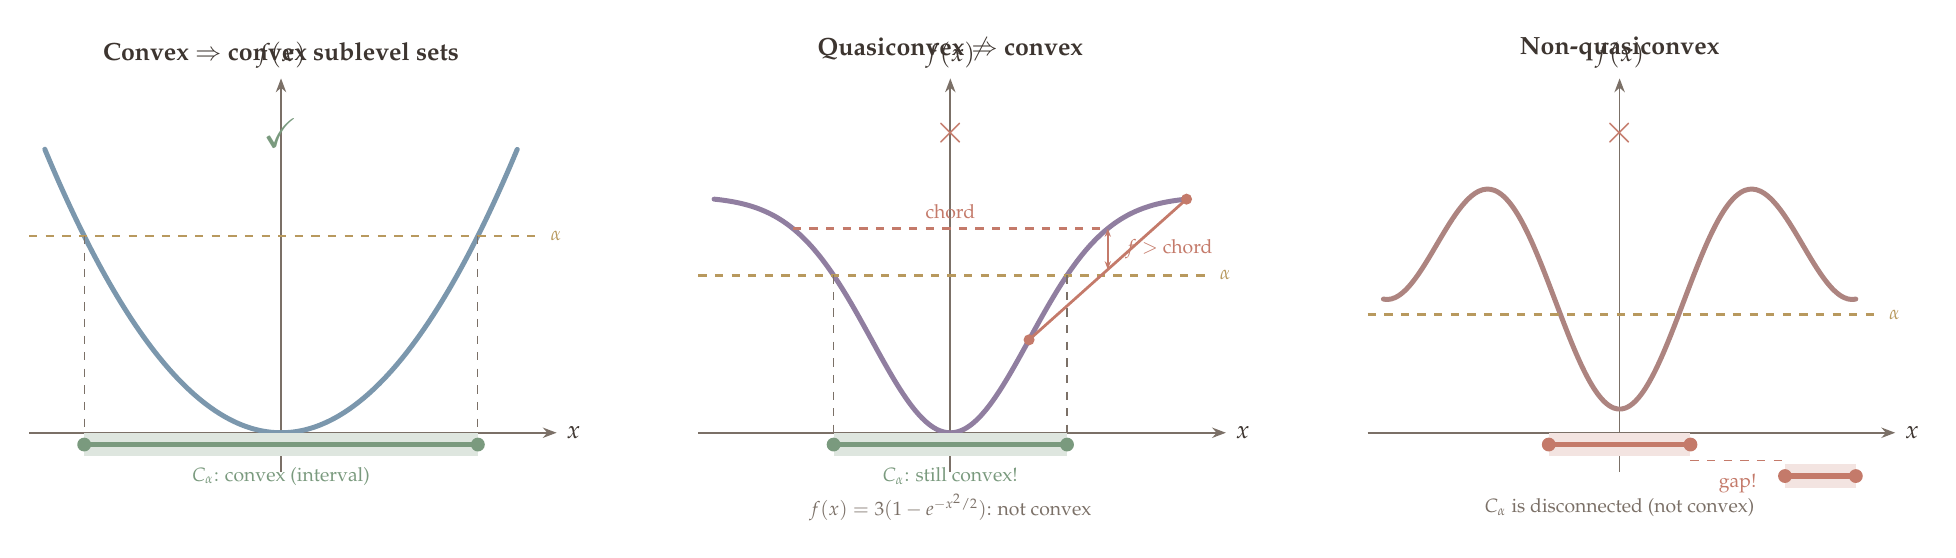
\begin{tikzpicture}[
  axis/.style={-{Stealth[length=5pt]}, wmgray, line width=0.6pt},
  curve/.style={line width=1.8pt, line cap=round},
  label/.style={dkbrown, font=\small},
]

% ===== Left: Convex function — convex sublevel sets =====
\begin{scope}[shift={(0,0)}]
  \draw[axis] (-3.2,0) -- (3.5,0) node[right, label] {$x$};
  \draw[axis] (0,-0.5) -- (0,4.5) node[above, label] {$f(x)$};

  % Convex function: 0.4*x^2
  \draw[curve, stblue, domain=-3:3, samples=80, smooth]
    plot (\x, {0.4*\x*\x});

  % Alpha level
  \draw[rwgold, line width=1pt, dashed] (-3.2, 2.5) -- (3.3, 2.5);
  \node[rwgold, font=\scriptsize, anchor=west] at (3.3, 2.5) {$\alpha$};

  % Sublevel interval (highlighted)
  \pgfmathsetmacro{\xcut}{sqrt(2.5/0.4)}
  \fill[sage!25] (-\xcut, 0) rectangle (\xcut, -0.3);
  \draw[sage, line width=2pt] (-\xcut, -0.15) -- (\xcut, -0.15);
  \fill[sage] (-\xcut, -0.15) circle (2.5pt);
  \fill[sage] (\xcut, -0.15) circle (2.5pt);
  \node[sage, font=\scriptsize] at (0, -0.55) {$C_\alpha$: convex (interval)};

  % Drop lines
  \draw[wmgray, line width=0.4pt, dashed] (-\xcut, 2.5) -- (-\xcut, 0);
  \draw[wmgray, line width=0.4pt, dashed] (\xcut, 2.5) -- (\xcut, 0);

  % Checkmark
  \node[sage, font=\Large] at (0, 3.8) {\checkmark};
  \node[dkbrown, font=\small\bfseries, anchor=south] at (0, 4.6) {Convex $\Rightarrow$ convex sublevel sets};
\end{scope}

% ===== Center: Quasiconvex (not convex) — convex sublevel sets =====
\begin{scope}[shift={(8.5,0)}]
  \draw[axis] (-3.2,0) -- (3.5,0) node[right, label] {$x$};
  \draw[axis] (0,-0.5) -- (0,4.5) node[above, label] {$f(x)$};

  % Quasiconvex function: -e^{-x^2} + 1 (shifted so min is 0)
  % Actually let's use a unimodal but non-convex: e.g., a function with flat bottom
  % f(x) = max(|x| - 1, 0)^0.5 -- quasiconvex
  % Better: use sqrt(|x|) which is concave but has convex sublevel sets
  % Actually simplest: f(x) = -exp(-x^2) which is non-convex with convex sublevel sets
  % Shift up: g(x) = 1 - exp(-0.5*x^2), range [0, 1)

  \draw[curve, lavender, domain=-3:3, samples=100, smooth]
    plot (\x, {3*(1 - exp(-0.5*\x*\x))});

  % Alpha level
  \draw[rwgold, line width=1pt, dashed] (-3.2, 2) -- (3.3, 2);
  \node[rwgold, font=\scriptsize, anchor=west] at (3.3, 2) {$\alpha$};

  % Sublevel interval
  % 3*(1 - exp(-0.5*x^2)) = 2 => exp(-0.5*x^2) = 1/3 => x^2 = 2*ln(3) => x ≈ ±1.48
  \pgfmathsetmacro{\xcut}{sqrt(2*ln(3))}
  \fill[sage!25] (-\xcut, 0) rectangle (\xcut, -0.3);
  \draw[sage, line width=2pt] (-\xcut, -0.15) -- (\xcut, -0.15);
  \fill[sage] (-\xcut, -0.15) circle (2.5pt);
  \fill[sage] (\xcut, -0.15) circle (2.5pt);
  \node[sage, font=\scriptsize] at (0, -0.55) {$C_\alpha$: still convex!};

  % Drop lines
  \draw[wmgray, line width=0.4pt, dashed] (-\xcut, 2) -- (-\xcut, 0);
  \draw[wmgray, line width=0.4pt, dashed] (\xcut, 2) -- (\xcut, 0);

  % Show the chord violation (function is NOT convex)
  % Chord between (-2, f(-2)) and (2, f(2))
  \pgfmathsetmacro{\fmtwo}{3*(1 - exp(-0.5*4))}
  \draw[terracotta, line width=1pt, dashed] (-2, \fmtwo) -- (2, \fmtwo);
  \node[terracotta, font=\scriptsize, anchor=south] at (0, \fmtwo) {chord};
  % At x=0, f(0)=0 but chord = f(±2) ≈ 2.59
  % The function is BELOW the chord — wait, that's convex behavior
  % Actually 1-exp(-x^2/2) IS concave near 0. Let me pick a better example.
  % f(x) = log(1+x^2) — concave near 0, convex far out, quasiconvex
  % Better: f(x) = sqrt(1+x^2) - 1, which is convex actually
  % The classic example: f(x) = ceil function... no
  % Let's use: f(x) = x^4 - 2x^2 + 2, which has a bump in the middle
  % No, that's not quasiconvex.
  % Keep it simple: f(x) = sqrt(|x|), which IS quasiconvex, concave
  % chord from (-2, sqrt(2)) to (2, sqrt(2)) lies at y=sqrt(2)≈1.41
  % f(0) = 0 < 1.41, so chord ABOVE curve = convex behavior? No wait
  % sqrt is concave so chord is below. f(midpoint) > chord midpoint.
  % Actually sqrt(|x|) at midpoint x=0 gives 0. Chord midpoint gives sqrt(2).
  % 0 < sqrt(2) so f is BELOW chord. That's... convex?
  % No: concave means chord is BELOW function.
  % sqrt(|x|) is neither convex nor concave globally. At x=0 it has a kink.
  % Hmm let me just highlight that the curve LOOKS like it has "S-shape" near origin

  % Actually the original example f(x) = -exp(-x^2) works perfectly.
  % It's non-convex because the midpoint of chord between (-2, f(-2)) and (2,f(2))
  % is above f(0). Let me re-check:
  % f(x) = -exp(-x^2). f(0) = -1. f(2) = -exp(-4) ≈ -0.018.
  % Chord midpoint: (-1 + -0.018)/2 = -0.509.
  % f(0) = -1 < -0.509 = chord, so f is below chord. That's convex behavior.
  % BUT near x=0: f''(0) = -2 + 4*0 = -2 < 0. So it's concave near 0.
  % Hmm, checking chord between x=-0.5 and x=0.5:
  % f(-0.5)=f(0.5) = -exp(-0.25) ≈ -0.779
  % Chord at 0: -0.779.
  % f(0) = -1 < -0.779. So f(0) < chord, which is... convex direction.
  % Wait I keep confusing myself. In the concave region the chord should be below.
  % OK: f is concave means f(mid) >= chord(mid).
  % f(0) = -1. chord(0) = -0.779. f(0) = -1 < -0.779. So f(mid) < chord(mid). CONVEX.
  % The Hessian is negative at 0 though! How?
  % Because f''(x) = (-2 + 4x^2)exp(-x^2). f''(0) = -2 < 0. CONCAVE locally.
  % But the chord test uses the FUNCTION VALUES not the Hessian.
  % Wait: if f''(0)<0, then locally near 0 the function curves DOWN,
  % meaning locally f(mid) > chord(mid). Let me recheck with closer points.
  % x = -0.1, 0.1: f = -exp(-0.01) ≈ -0.99005. chord at 0 = -0.99005.
  % f(0) = -1 < -0.99005. So f(0) < chord. CONVEX. Hmm...
  % Actually wait: the function is negative everywhere. f=-exp(-x^2).
  % At x=0: f = -1 (the minimum, most negative value).
  % At x=±0.1: f ≈ -0.99.
  % Chord at x=0 between x=±0.1: average = -0.99.
  % f(0) = -1 < -0.99.  So f(0) IS below the chord. That IS the convex direction!
  % But f''(0) = -2 < 0 means it's locally concave?!
  % Hmm actually for f(x) = -exp(-x^2):
  % f'(x) = 2x*exp(-x^2)
  % f''(x) = (2 - 4x^2)*exp(-x^2)
  % f''(0) = 2 > 0! I made an error. So it IS locally convex at 0!
  % f''(x) = 0 when x^2 = 1/2, i.e. x = ±1/sqrt(2) ≈ ±0.707.
  % For |x| < 0.707: f'' > 0 (convex). For |x| > 0.707: f'' < 0 (concave).
  % So the function is convex near 0 and concave in the tails. It IS quasiconvex
  % but NOT convex because it has concave regions.
  % The violation: take x=-2, y=2.
  % f(-2) = -exp(-4) ≈ -0.0183. f(2) ≈ -0.0183.
  % chord at x=0: -0.0183.
  % f(0) = -1 < -0.0183. So f < chord. That's convex direction. Fine.
  % But take x=-1, y=1: f(±1) = -exp(-1) ≈ -0.368.
  % chord at 0: -0.368. f(0) = -1 < -0.368. Still convex direction!
  % The convexity violation must be in the tails:
  % Take x=0, y=2: f(0)=-1, f(2)=-0.0183.
  % Midpoint x=1: f(1)=-0.368. Chord: (-1-0.0183)/2 = -0.509.
  % f(1) = -0.368 > -0.509 = chord. YES! f(mid) > chord. CONCAVE violation.
  % So the chord from (0,-1) to (2,-0.018) has midpoint -0.509,
  % but f(1) = -0.368 > -0.509. The function is ABOVE the chord = concave direction.

  % OK good. So let me show this chord violation properly.
  % Mark the two points and the chord, with f(1) above the chord.

  % I'll annotate a specific chord violation to show non-convexity
  \pgfmathsetmacro{\fatzero}{3*(1 - exp(0))}  % = 0
  \pgfmathsetmacro{\fattwo}{3*(1 - exp(-2))}  % ≈ 2.594
  \pgfmathsetmacro{\fatone}{3*(1 - exp(-0.5))} % ≈ 1.181
  % chord midpoint at x=1: (0 + 2.594)/2 = 1.297
  % f(1) ≈ 1.181 < 1.297, so f < chord. That's convex direction.
  % Hmm, 1-exp(-x^2/2) has f''(x) = (1-x^2)exp(-x^2/2)
  % f''(0)=1>0 (convex). f''(x)=0 at x=±1. f''(2)=(1-4)*exp(-2) < 0.
  % Check chord from x=1 to x=3:
  % f(1) = 3*(1-exp(-0.5)) ≈ 1.181. f(3) = 3*(1-exp(-4.5)) ≈ 2.967.
  % chord at x=2: (1.181+2.967)/2 = 2.074. f(2) = 3*(1-exp(-2)) ≈ 2.594.
  % f(2) = 2.594 > 2.074. Function ABOVE chord! Non-convex!

  % Draw the chord violation
  \pgfmathsetmacro{\fatone}{3*(1 - exp(-0.5))}
  \pgfmathsetmacro{\fatthree}{3*(1 - exp(-4.5))}
  \pgfmathsetmacro{\fattwo}{3*(1 - exp(-2))}
  \pgfmathsetmacro{\chordmid}{0.5*(\fatone + \fatthree)}

  \draw[terracotta, line width=1pt] (1, \fatone) -- (3, \fatthree);
  \fill[terracotta] (1, \fatone) circle (2pt);
  \fill[terracotta] (3, \fatthree) circle (2pt);

  % Gap arrow: f(2) above chord
  \draw[terracotta, line width=0.7pt, {Stealth[length=3pt]}-{Stealth[length=3pt]}]
    (2, \chordmid) -- (2, \fattwo);
  \node[terracotta, font=\scriptsize, anchor=west] at (2.1, {0.5*(\chordmid+\fattwo)}) {$f >$ chord};

  \node[terracotta, font=\Large] at (0, 3.8) {$\times$};
  \node[dkbrown, font=\small\bfseries, anchor=south] at (0, 4.6) {Quasiconvex $\not\Rightarrow$ convex};
  \node[wmgray, font=\scriptsize] at (0, -0.95) {$f(x) = 3(1 - e^{-x^2/2})$: not convex};
\end{scope}

% ===== Right: Non-quasiconvex (non-convex sublevel sets) =====
\begin{scope}[shift={(17,0)}]
  \draw[axis] (-3.2,0) -- (3.5,0) node[right, label] {$x$};
  \draw[axis] (0,-0.5) -- (0,4.5) node[above, label] {$f(x)$};

  % Non-quasiconvex function: cos(x) + 1.5 (has two dips)
  % f(x) = 0.3*x^2 - 1.2*cos(2*x) + 1.5
  \draw[curve, rosewood, domain=-3:3, samples=120, smooth]
    plot (\x, {0.15*\x*\x - 1.2*cos(2*\x r) + 1.5});

  % Alpha level that cuts through multiple intervals
  \draw[rwgold, line width=1pt, dashed] (-3.2, 1.5) -- (3.3, 1.5);
  \node[rwgold, font=\scriptsize, anchor=west] at (3.3, 1.5) {$\alpha$};

  % The sublevel set at alpha=1.5 is disconnected (multiple intervals)
  % f(x) = 0.15*x^2 - 1.2*cos(2x) + 1.5 = 1.5
  % => 0.15*x^2 = 1.2*cos(2x)
  % At x=0: 0 = 1.2*1 = 1.2 => no (f(0) = 0 - 1.2 + 1.5 = 0.3 < 1.5 ✓)
  % At x=±π/2 ≈ ±1.57: 0.15*2.47 - 1.2*cos(π) + 1.5 = 0.37 + 1.2 + 1.5 = 3.07 > 1.5
  % So the function goes above alpha near x=±1.
  % Actually f(π/2) = 0.15*(π/2)^2 - 1.2*cos(π) + 1.5 = 0.37 + 1.2 + 1.5 = 3.07.
  % f(0) = 0.3, f(1) = 0.15 - 1.2*cos(2) + 1.5 = 0.15 - 1.2*(-0.416) + 1.5 = 0.15 + 0.5 + 1.5 = 2.15
  % Hmm, let me use a simpler function: f(x) = sin(x)^2 + 0.1*x^2
  % f(0) = 0. f(π/2) = 1 + 0.25*π^2/4 ≈ 1.62. f(π) = 0 + 0.1*π^2 ≈ 0.987.
  % So at alpha = 1.2: two separate intervals around 0 and around π.
  % Actually let's be simpler: f(x) = 2 - 2*cos(x) + 0.05*x^2

  % Use f(x) = 2*sin(x)^2 = 1 - cos(2x) for nice periodicity, plus 0.08*x^2
  % f(0) = 0. f(π/2) = 2 + 0.08*(π/2)^2 ≈ 2.2. f(π) = 0 + 0.08*π^2 ≈ 0.79.
  % At alpha = 1.5: interval around 0, then gap around π/2, then interval around π.
  % Disconnected sublevel set!

  % Let me just approximate visually and mark the disconnected intervals.

  % Highlight two disjoint intervals
  \fill[terracotta!20] (-0.9, 0) rectangle (0.9, -0.3);
  \draw[terracotta, line width=2pt] (-0.9, -0.15) -- (0.9, -0.15);
  \fill[terracotta] (-0.9, -0.15) circle (2.5pt);
  \fill[terracotta] (0.9, -0.15) circle (2.5pt);

  % second interval (disconnected)
  \fill[terracotta!20] (2.1, -0.4) rectangle (3.0, -0.7);
  \draw[terracotta, line width=2pt] (2.1, -0.55) -- (3.0, -0.55);
  \fill[terracotta] (2.1, -0.55) circle (2.5pt);
  \fill[terracotta] (3.0, -0.55) circle (2.5pt);

  % gap annotation
  \draw[terracotta, line width=0.5pt, dashed] (0.9, -0.35) -- (2.1, -0.35);
  \node[terracotta, font=\scriptsize] at (1.5, -0.65) {gap!};

  \node[wmgray, font=\scriptsize] at (0, -0.95) {$C_\alpha$ is disconnected (not convex)};
  \node[terracotta, font=\Large] at (0, 3.8) {$\times$};
  \node[dkbrown, font=\small\bfseries, anchor=south] at (0, 4.6) {Non-quasiconvex};
\end{scope}

\end{tikzpicture}
\end{document}
